\documentclass[../main.tex]{subfiles}

\begin{document}

    \section{}

    \section{Exercices}

    \textbf{2.} La production privée de bien public, en l'absence de production publique est \ldots
        \begin{enumerate}
            \item Nulle
            \item Non nulle, sous optimale
            \item Optimale
	    \end{enumerate}

    \textbf{1.} Vaut-il mieux réguler les externalités négatives par les prix ou par les quantités ?

    \textbf{1.} Vaut-il mieux réguler les externalités négatives par les prix ou par les quantités ?

    \dotfill

    En l'absence d'incertitudes sur le point socialement optimal et de coûts de la régulation,
    les deux stratégies sont parfaitement équivalente.

    Si le régulateur peut se tromper sur le point socialement optimal, réguler par les prix
    implique que le prix de marché sera bien celui visé par le régulateur, mais que la quantité
    d'équilibre pourrait être très différente. Inversement, si la régulation se fait par les
    quantités, la quantité d'équilibre sera celle visée par le régulateur, mais le prix d'équilibre
    pourra être très différent du prix attendu. Ainsi, la régulation par les quantité est à privilégier
    dès lors que des petites erreurs sur les quantités ont des effets négatifs très importants.

    Par ailleurs, les coûts administratifs de collecte et/ou de contrôle peuvent être
    très différents selon la régulation choisie. Par exemple, il peut être moins coûteux de vérifier
    que les entreprises respectent certaines normes techniques que de mesurer directement
    la pollution qu'elles émettent. La meilleure régulation dépend donc des coûts
    de mise en place selon l'externalité qui est régulée.


    On considère une usine de l'industrie chimique dont la production  engendre
    des  rejets  polluants.

    Faites  l'hypothèse  que  la  demande  pour les produits de cette usine
    est  parfaitement  élastique.

    \textbf{1.} Représentez cette situation dans le plan (quantité, prix).

    \textbf{2.} L'équilibre de marché concurentiel est-il efficace dans cette
    situation ? Pourquoi ? Représentez le sur votre graphique.

    \textbf{3.} Expliquez  comment un régulateur public peut intervenir
    (de différentes façons) et quelles sont les limites de ces interventions.
    Représentez ces interventions.

    Les questions suivantes portent (entre autres) sur les documents joints aux exercices.

    \textbf{1.} En quoi consiste la contribution climat-énergie ?

    \textbf{2.} Quelle externalité vise-t-elle à corriger ? Comment une taxe
    peut-elle corriger une externalité négative ?

    \textbf{3.} Quels sont les effets redistributifs d'une taxe carbone ?

    \textbf{4.} Votre réponse à la question (3) dépend-elle de l'élasticité de
    la demande en énergie des ménages ? Si oui, comment ?

    \textbf{5.} Quelle utilisation des recettes de la taxe carbone vous semble
    être la plus juste ?

    \textbf{A.} \textit{6 points}

    On considère une usine de l'industrie chimique dont la production  engendre
    des  rejets  polluants.

    Faites  l'hypothèse  que  la  demande  pour les produits de cette usine
    est parfaitement  élastique.

    \textbf{1.} Représentez cette situation dans le plan (quantité, prix).

    \dotfill

    Voir figure 1 : il s'agit de représenter une courbe de demande compatible avec
    l'hypothèse sur son élasticité prix ; une courbe d'offre (c'est à dire de
    coût marginal) quelconque ; un dommage social marginal ; l'équilibre.
    
    \dotfill

    \begin{center}
    \begin{figure}[H]

    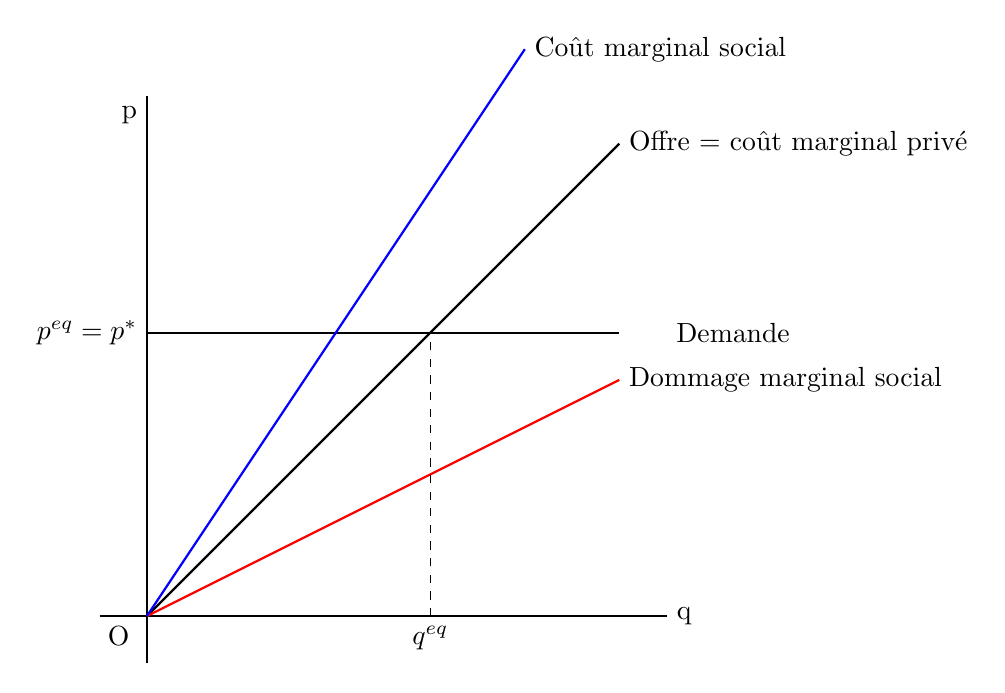
\begin{tikzpicture}[scale=1.2]

    \draw [thick] (-0.3,0) node [below] {O} (-0.5,0)-- (0,0) -- (5.5,0) node [right] {q};
    \draw [thick] (0,-0.5)-- (0,0) -- (0,5.5);
    \node [left] at (0,5.3) {p};

    \node [left] at (0,3) {$p^{eq} = p^{*}$};
    \node [right] at (5.5,3) {Demande};
    \draw [thick] (0,3) to (5,3);


    \draw [thick] (0,0) to (5,5);
    \node [right] at (5,5) {Offre $=$ coût marginal privé};

    \draw [thick, red] (0,0) to (5,2.5);
    \node [right] at (5,2.5) {Dommage marginal social};

    \draw [thick, blue] (0,0) to (4,6);
    \node [right] at (4,6) {Coût marginal social};

    \draw [dashed] (3,0) to (3,3);
    \node [below] at (3,0) {$q^{eq}$};

    \end{tikzpicture}

    \caption{Le marché de l'industrie chimique}

    \end{figure}
    \end{center}

    \dotfill

    \textbf{2.} L'équilibre de marché concurentiel est-il efficace dans cette
    situation ? Pourquoi ? Représentez le sur votre graphique.
    
    \dotfill
    
    L'équilibre de marché n'est pas efficace. Pour qu'il le soit, il faudrait qu'en
    ce point, le coût \textit{social} soit égal au bénéfice social. Or le point
    d'équilibre est tel que le coût \textit{privé} est égal au bénéfice \textit{privé}.
    Or ici les bénéfices privé et public ne coïncident pas, puisque la production
    de l'entreprise dégrade le bien-être des consommateurs. Le bénéfice privé est
    donc inférieur au bénéfice social, ou on peut considérer de manière équivalente
    que le coût social est supérieur au coût privé. Si l'on s'en tient à la deuxième
    interprétation, il y a sur-production parce que l'entreprise prend en compte un
    coût trop faible, et donc un point où coût et bénéfice sont égaux trop élevé.
    
    Cela se traduit par une perte sèche, qui correspond à toutes les unités produites
    telles que le coût social soit supérieur au bénéfice social. Elle est représentée
    par le triangle gris de la figure 2.
    
    \dotfill

    \begin{center}
    \begin{figure}[H]

    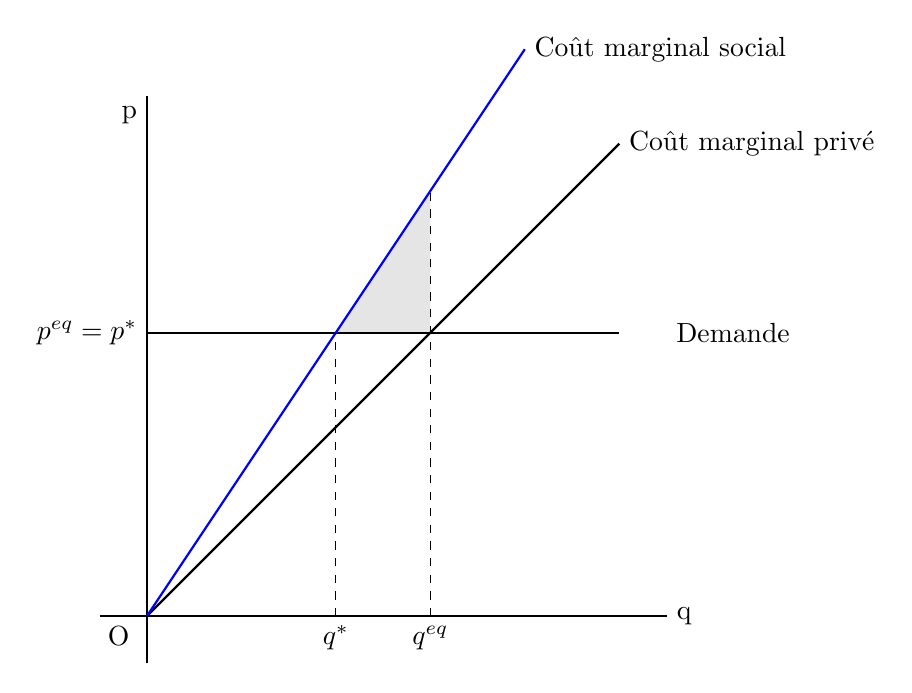
\begin{tikzpicture}[scale=1.2]

    \draw [thick] (-0.3,0) node [below] {O} (-0.5,0)-- (0,0) -- (5.5,0) node [right] {q};
    \draw [thick] (0,-0.5)-- (0,0) -- (0,5.5);
    \node [left] at (0,5.3) {p};

    \fill[fill = gray!20] (2,3) -- (3,4.5) -- (3,3) -- cycle;

    \node [left] at (0,3) {$p^{eq} = p^{*}$};
    \node [right] at (5.5,3) {Demande};
    \draw [thick] (0,3) to (5,3);


    \draw [thick] (0,0) to (5,5);
    \node [right] at (5,5) {Coût marginal privé};

    \draw [thick, blue] (0,0) to (4,6);
    \node [right] at (4,6) {Coût marginal social};

    \draw [dashed] (3,0) to (3,4.5);
    \node [below] at (3,0) {$q^{eq}$};
    
    \draw [dashed] (2,0) to (2,3);
    \node [below] at (2,0) {$q^{*}$};
    
    \end{tikzpicture}

    \caption{Le marché de l'industrie chimique}

    \end{figure}
    \end{center}


    \dotfill


    \textbf{3.} Expliquez  comment un régulateur public peut intervenir
    (de différentes façons) et quelles sont les limites de ces interventions.
    Représentez ces interventions.

    \dotfill
    
    Parmi les interventions possibles, on peut citer :
    \begin{itemize}
        \item D'instaurer une taxe par unité produite ou une subvention par unité non-produite,
        telle que la structure
        des coûts soit telle que l'équilibre corresponde à la situation
        optimale. Dans le cas d'une taxe, son montant doit être égal au
        dommage social marginal au point optimal, tel que le prix d'équilibre
        qui sera égal à la somme du coût privé et de la taxe soit égal au
        coût social. Voir figures 3 et 4. Les deux principales limites sont
        les effets redistributifs d'une telle taxe, et la difficulté à mesurer
        en pratique le dommage social marginal. La structure de la taxe / des subventions n'a pas d'effet
        sur l'efficacité tant qu'elle est égale, au point socialement efficace, au montant du dommage social
        marginal ; il s'agit simplement de transferts entre État, producteurs et consommateurs. Néanmoins,
        le régulateur pouvant se tromper sur la localisation de ce point optimale, le montant de la taxe 
        en dehors de ce point ne sera pas neutre. 
        \item D'agir directement sur les quantités, en fixant une limite à la production
        de l'entreprise. Il n'y a qu'une seule entreprise dans notre cas ; dans la réalité, se
        pose également la ventilation du quota total entre les différents producteurs.
        Déterminer la quantité optimale de biens à produire suppose également de connaître
        le dommage social marginal. Voir figure 5.
        \item D'assigner des droits de propriété sur l'air pur à l'entreprise ou aux individus,
        et de les laisser négocier le montant de pollution émis contre un dédomagement, c'est
        à dire supprimer l'externalité en créant un marché pour celle-ci. Cela n'est possible
        que si la négociation est possible, ce qui n'est pas le cas lorsque le nombre d'agents
        est important.
        \item D'internaliser l'externalité en organisant le rachat de l'entreprise par les
        individus concernés par la pollution, auquel cas il n'y a plus d'externalité puisque
        l'agent qui la subit (les individus) et l'agent qui la produit (également les individus)
        est le même.
        \item De mettre en place des normes contraignantes sur la production, c'est à dire d'augmenter
        le coût privé pour diminuer le dommage social marginal, en laissant le coût marginal social inchangé.
        Cela revient à forcer l'entreprise à internaliser l'externalité en changeant sa technologie. Cela suppose
        naturellement que le régulateur connaîsse la technologie optimale à mettre en place pour
        réduire le dommage social à moindre coût. Voir figure 6.
    \end{itemize}
    
    \dotfill

    \begin{center}
    \begin{figure}[H]

    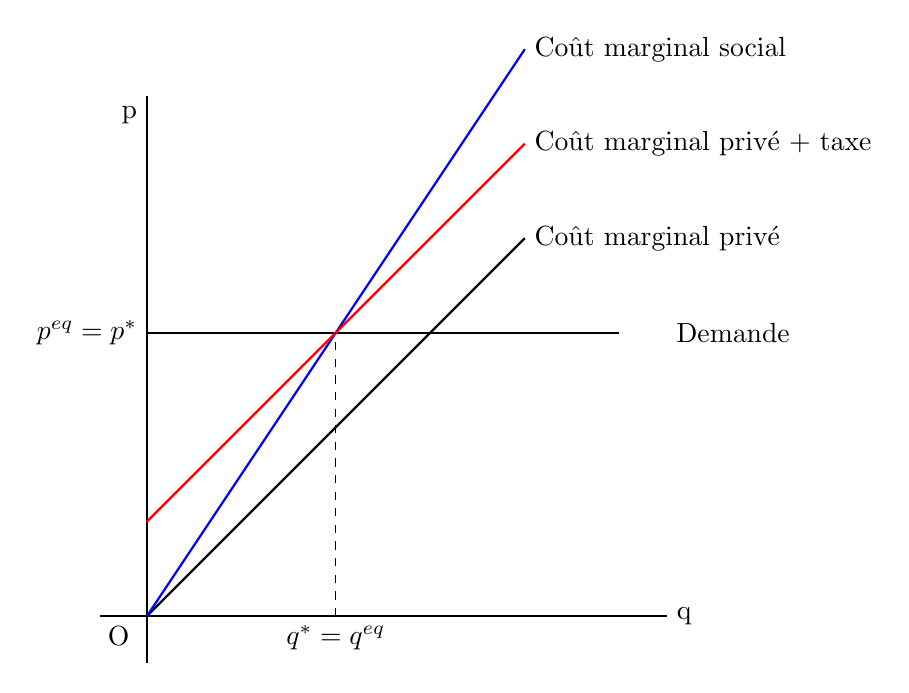
\begin{tikzpicture}[scale=1.2]

    \draw [thick] (-0.3,0) node [below] {O} (-0.5,0)-- (0,0) -- (5.5,0) node [right] {q};
    \draw [thick] (0,-0.5)-- (0,0) -- (0,5.5);
    \node [left] at (0,5.3) {p};


    \node [left] at (0,3) {$p^{eq} = p^{*}$};
    \node [right] at (5.5,3) {Demande};
    \draw [thick] (0,3) to (5,3);

    \draw [thick] (0,0) to (4,4);
    \node [right] at (4,4) {Coût marginal privé};

    \draw [thick, blue] (0,0) to (4,6);
    \node [right] at (4,6) {Coût marginal social};

    \draw [thick, red] (0,1) to (4,5);
    \node [right] at (4,5) {Coût marginal privé $+$ taxe };

    \draw [dashed] (2,0) to (2,3);
    \node [below] at (2,0) {$q^{*} = q^{eq}$};
    
    \end{tikzpicture}

    \caption{Régulation par les prix}

    \end{figure}
    \end{center}


    \begin{center}
    \begin{figure}[H]

    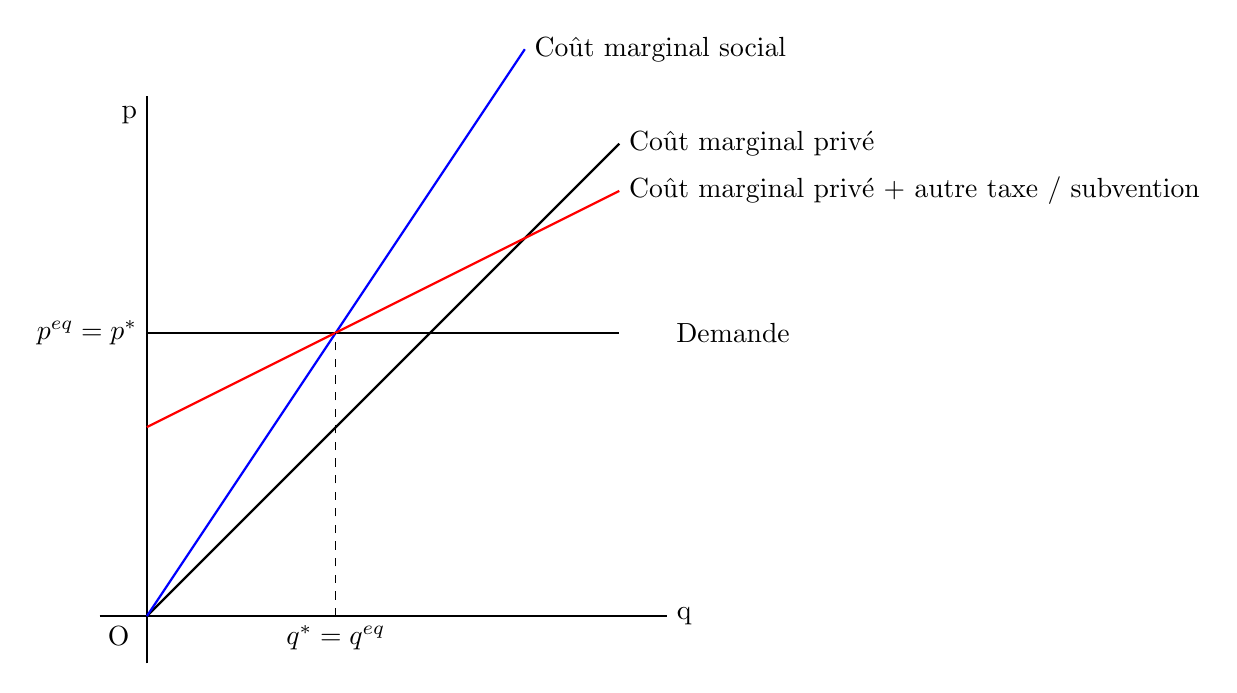
\begin{tikzpicture}[scale=1.2]

    \draw [thick] (-0.3,0) node [below] {O} (-0.5,0)-- (0,0) -- (5.5,0) node [right] {q};
    \draw [thick] (0,-0.5)-- (0,0) -- (0,5.5);
    \node [left] at (0,5.3) {p};


    \node [left] at (0,3) {$p^{eq} = p^{*}$};
    \node [right] at (5.5,3) {Demande};
    \draw [thick] (0,3) to (5,3);

    \draw [thick] (0,0) to (5,5);
    \node [right] at (5,5) {Coût marginal privé};

    \draw [thick, blue] (0,0) to (4,6);
    \node [right] at (4,6) {Coût marginal social};

    \draw [thick, red] (0,2) to (5,4.5);
    \node [right] at (5,4.5) {Coût marginal privé $+$ autre taxe / subvention };

    \draw [dashed] (2,0) to (2,3);
    \node [below] at (2,0) {$q^{*} = q^{eq}$};
    
    \end{tikzpicture}

    \caption{Régulation par les prix}

    \end{figure}
    \end{center}

    \begin{center}
    \begin{figure}[H]

    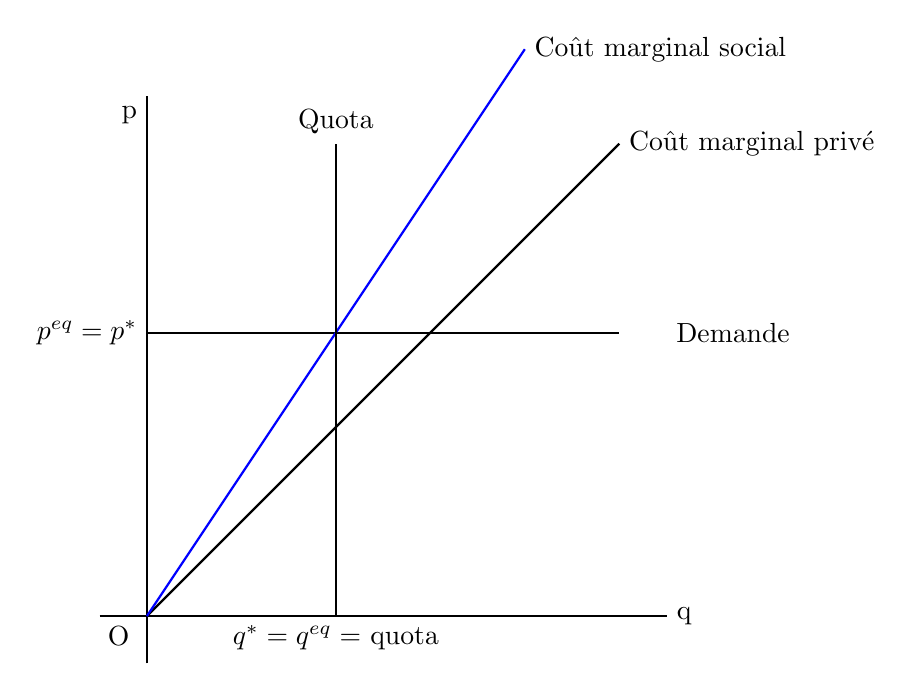
\begin{tikzpicture}[scale=1.2]

    \draw [thick] (-0.3,0) node [below] {O} (-0.5,0)-- (0,0) -- (5.5,0) node [right] {q};
    \draw [thick] (0,-0.5)-- (0,0) -- (0,5.5);
    \node [left] at (0,5.3) {p};


    \node [left] at (0,3) {$p^{eq} = p^{*}$};
    \node [right] at (5.5,3) {Demande};
    \draw [thick] (0,3) to (5,3);

    \draw [thick] (0,0) to (5,5);
    \node [right] at (5,5) {Coût marginal privé};

    \draw [thick, blue] (0,0) to (4,6);
    \node [right] at (4,6) {Coût marginal social};

    \draw [dashed] (2,0) to (2,3);
    \draw [thick] (2,0) to (2,5);
    \node [above] at (2,5) {Quota};
    \node [below] at (2,0) {$q^{*} = q^{eq} =$ quota};
    
    \end{tikzpicture}

    \caption{Régulation par les quantités}

    \end{figure}
    \end{center}

    \begin{center}
    \begin{figure}[H]

    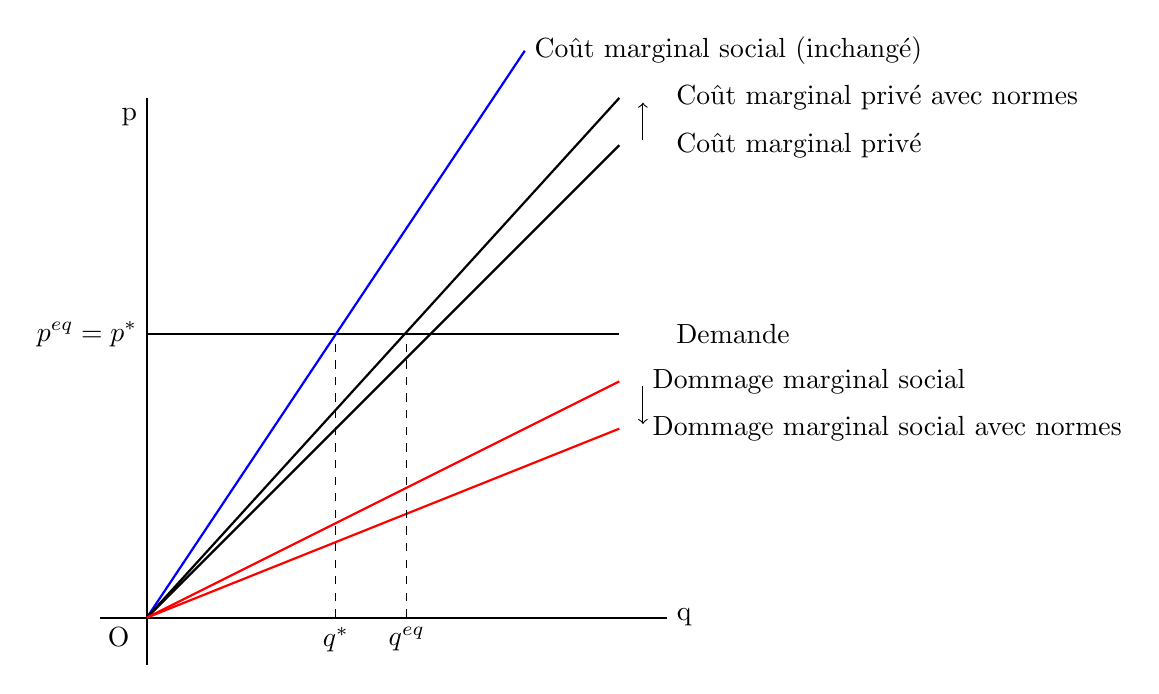
\begin{tikzpicture}[scale=1.2]

    \draw [thick] (-0.3,0) node [below] {O} (-0.5,0)-- (0,0) -- (5.5,0) node [right] {q};
    \draw [thick] (0,-0.5)-- (0,0) -- (0,5.5);
    \node [left] at (0,5.3) {p};


    \node [left] at (0,3) {$p^{eq} = p^{*}$};
    \node [right] at (5.5,3) {Demande};
    \draw [thick] (0,3) to (5,3);

    \draw [thick, blue] (0,0) to (4,6);
    \node [right] at (4,6) {Coût marginal social (inchangé)};

    \draw [thick] (0,0) to (5,5);
    \node [right] at (5.5,5) {Coût marginal privé};

    \draw [->] (5.25, 5.05) -- (5.25, 5.45);

    \draw [thick] (0,0) to (5,5.5);
    \node [right] at (5.5,5.5) {Coût marginal privé avec normes};
    
    \draw [thick, red] (0,0) to (5,2.5);
    \node [right] at (5.25,2.5) {Dommage marginal social};

    \draw [->] (5.25, 2.45) -- (5.25, 2.05);

    \draw [thick, red] (0,0) to (5,2);
    \node [right] at (5.25,2) {Dommage marginal social avec normes};

    \draw [dashed] (2.75,0) to (2.75,3);
    \node [below] at (2.75,0) {$q^{eq}$};
    
    \draw [dashed] (2,0) to (2,3);
    \node [below] at (2,0) {$q^{*}$};

    
    \end{tikzpicture}

    \caption{Régulation par les normes techniques}

    \end{figure}
    \end{center}

    \textbf{A.} Biens publics \textit{12 points}

    On étudie le modèle de Knight, 2003 (section 3).

    On se place dans le cas d'une économie où deux biens existent : un bien
    privé~\(c\) et un bien public~\(g\). Cette économie est composée d'un seul type d'individus, au nombre de
    \(N\). On suppose que leur utilité est, pour un individu~\(i\)~:
    \[U_{i}\left(c_{i}, g\right) = h\left(g\right) + c_{i} \]

    On suppose enfin que chaque individu possède \(m\) unités du
    bien privé \(c\) et que l'on peut produire une unité de bien public
    avec une unité de bien privé.

    \textbf{1.} Rappelez ce qu'est un taux marginal de substitution technique.
    Quel est le taux marginal de substitution technique entre le bien privé et
    le bien public ?

    On considère un planificateur social qui souhaite maxmimiser la somme des
    utilités des individus.

    \textbf{2.} Exprimez la fonction de bien être social en fonction de \(g\)
    et des \(c_{i}\). La distribution des \(c_{i}\) a-t-elle un effet sur la
    fonction de bien-être social ?

    On note \(C = \sum_{i} c_{i} \).

    \textbf{3.} Quelle est la contrainte budgétaire du planificateur social ?
    Autrement dit, quelle est la relation entre \(C\) et \(g\) ?

    \textbf{4.} Retrouvez l'équation (2) de l'article en maximisant la fonction de
    bien-être social. Comment se nomme cette relation et comment
    s'interpète-t'elle ?

    \textbf{5.} À partir de l'équation (3), de la variable de choix du
    législateur (voter pour \(L\) ou pour \(R\)), et de l'hypothèse \(g^{R} =
    0\), retouvez l'inéquation (4).

    \textbf{7.} Pourquoi la dépense dans chaque circonscription n'est-elle pas égale à la dépense optimale ?
    
    \textbf{6.} Quelle est la perte sèche totale due aux circonscriptions recevant un
    financement insuffisant ? Quelle est la perte sèche totale due aux districts
    recevant un financement excessif ?
    


    \textbf{A.} Biens publics \textit{12 points}

    On étudie le modèle de Knight, 2003 (section 3).

    On se place dans le cas d'une économie où deux biens existent : un bien
    privé~\(c\) et un bien public~\(g\). Cette économie est composée d'un seul type d'individus, au nombre de
    \(N\). On suppose que leur utilité est, pour un individu~\(i\)~:
    \[U_{i}\left(c_{i}, g\right) = h\left(g\right) + c_{i} \]

    On suppose enfin que chaque individu possède \(m\) unités du
    bien privé \(c\) et que l'on peut produire une unité de bien public
    avec une unité de bien privé.

    \textbf{1.} Rappelez ce qu'est un taux marginal de substitution technique.
    Quel est le taux marginal de substitution technique entre le bien privé et
    le bien public ?

    \dotfill

    Le taux marginal de substitution technique entre deux facteurs représente le
    sacrifice dun facteur auquel il faut consetir pour utiliser une unité
    supplémentaire de l'autre facteur tout en restant au même niveau de
    production. Analytiquement, c'est le ratio des productions marginales.
    Graphiquement, il correspond à la pente de la tangente à l'isoquante.

    Dans notre cas, il s'agit de la quantité de bien privé qui doit être
    sacrifiée pour produir eune unité supplémentaire de bien public.

    Par hypothèse, \(TMT_{g, c} = 1\).

    \dotfill

    On considère un planificateur social qui souhaite maxmimiser la somme des
    utilités des individus.

    \textbf{2.} Exprimez la fonction de bien être social en fonction de \(g\)
    et des \(c_{i}\). La distribution des \(c_{i}\) a-t-elle un effet sur la
    fonction de bien-être social ?

    \dotfill

    La somme des utilités individuelles est :
    \[ SWF = \sum_{i=1}^{N} U_{i} = \sum_{i=1}^{N} \left( h\left(g\right) +
    c_{i} \right) = \sum_{i=1}^{N} h\left(g\right) + \sum_{i=1}^{N} c_{i}
    = Nh\left(g\right) + \sum_{i=1}^{N} c_{i} = Nh\left(g\right) + C \]

    La distribution des \(c_{i}\) n'a aucune conséquence sur la fonction de
    bien-être social.

    Prenons le cas de deux individus, \(k\) et \(l\) et transférons une quantité
    \(\phi\) de consommation de \(k\) vers \(l\).

    En notant \(SWF^{av}\) la valeur de la fonction de bien-être social
    avant le transfert et \(SWF^{ap}\) la valeur de la fonction de bien-être
    social après le transfert, on a :
    \begin{align*}
        SWF^{ap} &= Nh\left(g\right) + \left(\sum_{i \neq k, i \neq l} c_{i} \right) + \left(c_{k} -
        \phi\right) + \left(c_{l} + \phi\right) \\
                 &= Nh\left(g\right) + \left(\sum_{i \neq k, i \neq l} c_{i} \right) + c_{k} +
        c_{l} + \phi - \phi \\
                 &= Nh\left(g\right) + \left(\sum_{i \neq k, i \neq l} c_{i} \right) + c_{k} +
        c_{l} \\
                 &= Nh\left(g\right) + \sum_{i=1}^{N} c_{i}  \\
                 &= SWF^{av} \\
    \end{align*}

    \dotfill

    On note \(C = \sum_{i} c_{i} \).

    \textbf{3.} Quelle est la contrainte budgétaire du planificateur social ?
    Autrement dit, quelle est la relation entre \(C\) et \(g\) ?

    \dotfill

    Par hypothèse, chaque individu possède \(m\) unités du bien privé.

    La quantité totale de bien privé est donc de \(Nm\).

    Puisque l'on peut utiliser une unité de bien privé pour produire une unité
    de bien public, on a donc la relation :
    \[ g + C \leq Nm \]

    \dotfill

    \textbf{4.} Retrouvez l'équation (2) de l'article en maximisant la fonction de
    bien-être social. Comment se nomme cette relation et comment
    s'interpète-t'elle ?

    \dotfill

    On susbtitute la contrainte de budget dans la fonction de bien-être social :
    \begin{align*}
        SWF &= Nh\left(g\right) + C \\
            &= Nh\left(g\right) + Nm - g
    \end{align*}

    Au maximum, on a :
    \[ \frac{dSWF}{dg} = 0 \Rightarrow Nh'\left(g\right) - 1 = 0 \Rightarrow
    Nh'\left(g\right)= 1 \]

    On retrouve bien la condition de de Samuelson : à l'optimum, la somme des
    taux marginaux de substitution du bien public par rapport au bien privé (terme de gauche)
    est égale au taux marginal de substitution technique (terme de droite).

    Autrement dit, le bénéfice social d'une unité supplémentaire de bien public
    et d'une unité en moins de bien privé est égal au coût en unité de bien
    privé de produire une unité de bien public supplémentaire.

    \dotfill

    \textbf{5.} À partir de l'équation (3), de la variable de choix du
    législateur (voter pour \(L\) ou pour \(R\)), et de l'hypothèse \(g^{R} =
    0\), retouvez l'inéquation (4).

    \dotfill

    Le représentant vote pour (respectivement, contre) le budget si l'utilité
    procurée par le budget proposé (avec un niveau de dépense publique dans sa
    circonscription de \(g^{L}\) et une dépense totale de \(G^{L}\)) est supérieure
    (resp.\ inférieure) à l'utilité procurée par le budget par défaut où
    \(g^{R} = 0\) et \(G^{R} = 0\)

    On note \(\tau = \frac{G}{J}\) la part de la dépense totale payée par la
    circonscription du représentant considéré (cf.\ page 5).

    Alors, le représentant vote pour le budget lorsque :
    \begin{align*}
                    & U^{L} \geq U^{R} \\
        \Rightarrow & h\left(g^{L}\right) + m_{j} - \frac{G^{L}}{NJ} \geq
        h\left(g^{R}\right) + m_{j} - \frac{G^{R}}{NJ} \\
        \Rightarrow & h\left(g^{L}\right) + m_{j} - \frac{G^{L}}{NJ} \geq
        h\left(0\right) + m_{j} - \frac{0}{NJ} \\
        \Rightarrow & h\left(g^{L}\right) + m_{j} - \frac{G^{L}}{NJ} \geq
        0 + m_{j} - 0 \\
        \Rightarrow & h\left(g^{L}\right) + m_{j} - \frac{G^{L}}{NJ} \geq
        m_{j} \\
        \Rightarrow & h\left(g^{L}\right) - \frac{G^{L}}{NJ} \geq 0 \\
        \Rightarrow & h\left(g^{L}\right) \geq \frac{G^{L}}{NJ} \\
        \Rightarrow & h\left(g^{L}\right) \geq \frac{\tau}{N} \\
    \end{align*}

    \dotfill

    \textbf{7.} Pourquoi la dépense dans chaque circonscription n'est-elle pas égale à la dépense optimale ?

    \dotfill

    Il ya deux effets en jeu :
    \begin{itemize}
        \item Puisque chaque circonscription ne paye qu'une partie des coûts associés
              à la production de bien public chez elle, le point où le coût privé est égal
              au bénéfice privé correspond à une quantité plus importante de bien public
              que le point où le coût social est égal au bénéfice social (ce dernier étant égal
              au bénéfice privé).
        \item Puisqu'il n'est nécessaire d'obtenir que l'accord d'une majorité des circonscriptions
              et non l'unanimité, la coalition gagnante peut choisir une sur-allocation pour les membres
              de la coalition et une sous-allocation pour les autres, tout en restant majoritaire. 
    \end{itemize}

    \dotfill

    \textbf{6.} Quelle est la perte sèche totale due aux circonscriptions recevant un
    financement insuffisant ? Quelle est la perte sèche totale due aux districts
    recevant un financement excessif ?

    \dotfill

    Cf. table 1.

    \dotfill
\end{document}
